\chapter{Resultados} \label{ch:Resultados}
	%  Os resultados seguem a metodologia

	% Definir qual o top_k utilizado
	% Verificar em Were2014 novamente
	% Padrão do zettair (se não me engano é 20)
	% Artigo de fulano não diz

	% Capítulo de Resultados 

	% -> Introdução: "Este capítulo apresenta os resultados obtidos e discute-os..." 
	Este capítulo apresenta os resultados obtidos neste estudo investigativo do desempenho de atributos de RI em classificadores de Mineração de Texto.

	Nas subseções a seguir primeiro é abordada a configuração experimental utilizada para realizar o estudo, e logo em seguida é apresentada uma visão geral das soluções selecionadas dos corpus DB\underscore{}AUTHORPROF e DB\underscore{}HYPERPARTISAN, na qual o pré-processamento realizado e os classificadores utilizados em cada uma das soluções são descritos brevemente.
	Por fim, são apresentados os resultados mensurados por meio das medidas escolhidas para avaliação de desempenho, na Seção \ref{sec:DesempenhoFerramentas} estão as medidas de desempenho das ferramentas de armazenamento e indexação, e na Seção \ref{sec:DesempenhoClassificadores} são expostas as medidas de desempenho dos classificadores.

	% Na subseção a seguir são abordados os resultados referentes às ferramentas de indexação.
	% Na subseção posterior são abordados os resultados referente aos desempenho das variáveis de RI em classificadores.

	\section{Configuração experimental} \label{sec:ConfiguraçãoExperimental}
	% 4.0 Setup experimental 

		Para programação e execução dos experimentos foi utilizado o sistema computacional disponível para o autor, com a configuração disposta na Tabela \ref{tab:sistema-computacional}.

		\begin{table}[ht]
    \centering
    \caption{Configuração do computador de mesa utilizado neste estudo.}
    \begin{adjustbox}{max width={\textwidth},keepaspectratio}%
    \begin{tabular}{|l|l|}
        \hline
        % \textbf{Posição}  
        % & \makecell[l]{\textbf{Equipe}}
        % & \makecell[l]{\textbf{Repositório de código no site \url{https://github.com/}}}
        % \\ \hline
        Processador
        & Intel(R) Core(TM) i7-4770 CPU @ 3.40GHz
        \\ \hline
        Memória RAM
        & 32370 MB
        \\ \hline
        Sistema Operacional
        & Linux Mint 19.2 Tina
        \\ \hline
        Placa-mãe
        & Gigabyte Z97-D3H
        \\ \hline
        Gráficos
        & Mesa DRI Intel(R) Haswell Desktop
        \\ \hline
        Disco
        & HP SSD EX920 512GB
        \\ \hline
    \end{tabular}
    \end{adjustbox}
    \legend{\ABNTEXfontereduzida \textbf{Fonte:} O autor.}
    \label{tab:sistema-computacional}
\end{table}
		
		As ferramentas de armazenamento e indexação receberam os mesmos parâmetros de refinamento na configuração de suas funções BM25, sendo estes configurados em $k_1 = 1.2$, $k_3 = 0$ e $b = 0.75$.
		O parâmetro $k_3$ (escalonar frequência de termos na consulta) é exclusivo do Zettair, as demais ferramentas não implementam este parâmetro.

		% Fixação do número aleatório do Python e das bibliotecas utilizadas nas soluções, quando isto não era feito originalmente, para permitir reprodutibilidade exata dos resultados obtidos.
		% [ ] FOOTNOTE DO VSCODIUM?
		O ambiente de programação utilizado foi o VSCodium e a linguagem de programação utilizada foi o Python 3.7.5.
		Para permitir reprodutibilidade dos resultados obtidos, o gerador de números aleatórios (RNG) do ambiente do Python, assim como os RNGs das bibliotecas utilizadas pelas soluções, tiveram as suas sementes de geração fixadas.

		Todos os códigos fontes dos scripts Python criados para este estudo estão disponíveis em um repositório de código online e público criado pelo autor, acessível pelo seguinte link: \url{https://github.com/ruanmed/tcc-ii-ir-features-text-mining/}.
		A seguir são tratadas as dependências de \textit{software} para execução do estudo.

		\subsection{Dependências de \textit{software}} \label{subsec:DependênciasSoftware}
			Para execução dos scripts Python gerados por esse estudo é necessário Python >= 3.6 com as bibliotecas elasticsearch-py >= 7.0.5 e python-arango >= 5.2.1.
			Ambas bibliotecas se encontram disponíveis no PyPI (\textit{Python Package Index}, ou índice de pacotes do Python em tradução livre).

			Também é necessário possuir instâncias do Elasticsearch >= 7.4.0 e do ArangoDB >= 3.5.1 rodando e disponíveis na rede local do sistema, isso pode ser feito por meio da instalação dessas ferramentas no sistema local.
			O Zettair >= 0.94 também é necessário estar instalado no sistema, sendo possível executá-lo pelo terminal de comandos com o comando 'zet'.

			A instalação das três ferramentas em sistemas Linux foi simplificada com a criação de um arquivo Docker que utiliza de imagens disponíveis online do ArangoDB e do Elasticsearch, reduzindo o número de comandos necessários para executar as ferramentas no sistema computacional.
			Detalhes de como utilizar esse arquivo Docker se encontram em: \url{https://github.com/ruanmed/tcc-ii-ir-features-text-mining\#docker-file}.

			Além dessas dependências, é necessário também instalar as bibliotecas específicas de cada uma das soluções selecionadas.
			Essas estão listadas nos arquivos README disponibilizados junto às soluções.

	\section{Visão geral das soluções selecionadas e adaptações feitas} \label{sec:VisãoSoluçõesEAdaptações}
		% Falar brevemento sobre o pré-processamento;
		% Falar sobre o classificador utilizado; e
		% Indicar o Notebook de cada solução para mais detalhes
		As soluções selecionadas para reprodução e posterior adição dos atributos de RI utilizam de diferentes técnicas para pré-processamento dos corpus e também de classificadores diferentes, tornando necessário, em alguns casos, ajustes antes da adição dos atributos de RI.

		Nas subseções a seguir são brevemente abordadas as soluções 1\underscore{}bertha e 4\underscore{}tom do corpus DB\underscore{}HYPARTISAN, e a solução 2\underscore{}daneshvar18 do corpus DB\underscore{}AUTHORPROF.

		\subsection{Corpus DB\underscore{}HYPERPARTISAN}
			O corpus DB\underscore{}HYPERPARTISAN possui dois conjuntos de dados, o primeiro com 750 mil artigos classificados por enviesamento do editor, e o segundo com 645 artigos rotulados como hiperpartidários ou não com consenso entre avaliadores via \textit{crowdsourcing}.
			O objetivo da competição que utilizou esse corpus era classificar artigos como hiperpartidários ou não, e assim os participantes puderam utilizar os dois conjuntos para fazer suas avaliações. 
			No entanto, a utilização dos 750 mil artigos classificados por enviesamento de editor não foram úteis para ajudar na classificação, e das duas soluções selecionadas nenhuma delas utilizou esses 750 mil artigos nos seus modelos finais, pois utilizar a informação de editor em conjunto reduziu o desempenho de seus classificadores \cite[p.~840]{jiang-etal-2019-team} pois segundo \citeonline[p.~1067]{yeh-etal-2019-tom} o conjunto de dados classificado por enviesamento do editor possui muito ruído.
			% Nota de rodapé sobre ruído

			O conjunto de validação final da competição, com 628 artigos também classificados manualmente, não foi disponibilizado ao público, portanto para reprodução das soluções foi necessário dividir o conjunto de 645 artigos em treinamento e validação pelo método de \textit{holdout}, ficando assim com 430 artigos para treinamento e 215 artigos para teste. 
			Essa divisão foi feita de modo que as classes mantiveram-se com o mesmo balanceamento do conjunto original (37\% dos artigos hiperpartidário e 63\% não hiperpartidários).

			Então, os 430 artigos foram indexados em todas as ferramentas de indexação permitindo a posterior geração dos atributos de RI.
			A indexação foi feita com auxílio da classe \textit{IndexToolManager} criada pelo autor, que é abordada com detalhes na seção de desempenho das ferramentas de armazenamento e indexação.
			
			\subsubsection{Solução 1\underscore{}bertha}
				A solução da equipe Bertha von Suttner (4\underscore{}bertha) para essa tarefa da \textit{SemEval 2019} consiste em uma abordagem de classificação com uma Rede Neural Convolucional (\textit{Convolutional Neural Network}, CNN) e o pré-processamento dos documentos do corpus em uma representação destes por meio de uma Rede ESRC (\textit{ELMo Sentence Representation Convolutional Network}), uma representação sugerida e nomeada pela equipe.

				A representação na Rede ESRC é uma alternativa à representação usual dos documentos por termos (ou \textit{tokens}).
				Essa representação consiste no cálculo da média dos agregados ELMo para os documentos, a nível de frase, e cada documento é representado como uma sequência desses agregados, que são vetores de tamanho de 1024 \textit{floats}. 
				Na implementação da solução cada documento é limitado a ocupar até 200 vetores de tamanho 1024, sendo então cada documento padronizado com forma 200 x 1024.
				ELMo é uma representação de palavras com contextualização profunda, que modela características complexas de uso das palavras, como sintaxe e semântica, e o uso dessas palavras em contextos linguísticos \cite{ELMoDBLP:journals/corr/abs-1802-05365}.

				A CNN do classificador consiste de 5 camadas convolucionais paralelas internamente que recebem como entrada os agregados ELMo, essas 5 camadas convolucionais se conectam a camada de saída da rede neural, com função de ativação sigmoid, mais detalhes da implementação da CNN podem ser vistos em \citeonline{jiang-etal-2019-team}.

				Para adicionar os 6 atributos de RI à rede foram embutidos, ao final de cada representação de documento, 6 vetores de tamanho 1024, preenchidos pelo valor calculado de cada atributo para o respectivo documento, resultando em documentos com forma 206 x 1024.
				A adaptação da solução está ilustrada na Figura \ref{fig:1-bertha-arquitetura-com-ri}.
				
				\begin{figure}[ht]
    \centering
    \caption{Arquitetura de sistema da solução 1\underscore{}bertha após adaptação.}
    \begin{center}
        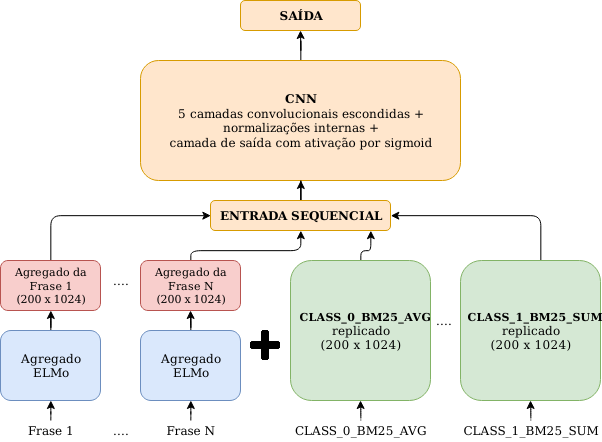
\includegraphics[width=0.75\textwidth]{img/1-bertha-arquitetura-com-ri.png}
    \end{center}
    \vspace{-0.5cm}
    \legend{\ABNTEXfontereduzida \textbf{Fonte:} O autor.}
    \label{fig:1-bertha-arquitetura-com-ri}
\end{figure}

				% \ref{fig:1-bertha-arquitetura-com-ri}
				A Figura \ref{fig:1-bertha-arquitetura-com-ri} é baseada na figura de representação de arquitetura do sistema apresentada no artigo de descrição da solução da equipe \cite{jiang-etal-2019-team}, alguns detalhes da CNN são abstraídos e os atributos de RI adicionados estão representados em verde.

				% Tem que adicionar aqui sobre o modo que a solução faz a predição

			\subsubsection{Solução 4\underscore{}tom}
				A solução da equipe Tom Jumbo-Grumbo (4\underscore{}tom) utilizou de dois classificadores, um de Regressão Logística e outro de Máquinas de Vetor de Suporte (SVMs), sendo o utilizado no modelo final o classificador SVC (C-Support Vector Classification) da biblioteca sklearn para Python.
				Uma SVM funciona transformando os dados de treinamento para uma dimensão maior e então executa uma busca pelo melhor limite de decisão, chamado de hiperplano, para separar as classes \cite[p.~408]{Han:2011:DMC:1972541}.
				Em especial, o classificador SVC da biblioteca sklearn possui um parâmetro de regularização de sua função de custo (parâmetro chamado de C) que deve ser estritamente positivo, o valor padrão é definido como $C = 1,0$, no entanto a solução da equipe, conforme disposto no código fonte disponível online, utilizou $C = 0,9$ após uma análise com diferentes valores.

				No pré-processamento, a equipe utilizou três estratégias para converter os documentos em atributos para o classificador.
				A primeira foi de criar vetores baseados na frequência dos termos, descartando termos que apareçam em mais de 90\% dos documentos e utilizando os 50 mil termos mais frequentes dos que sobrarem, guardando o valor tf-idf para cada termo respectivo ao documento.
				A segunda foi treinar um modelo PV-DM para gerar os atributos referentes a cada documento.
				E a terceira utilizou um agregado pré-treinado em textos da Wikipédia com o algoritmo GloVe, que, similarmente aos agregados ELMo, tentam também inferir o significado das palavras dos documentos.

				A arquitetura com melhor resultado foi a utilização dos atributos GloVe com o classificador SVM da biblioteca sklearn.
				Os documentos são convertidos para os vetores GloVe pré-treinados a partir se suas primeiras 1000 palavras, esses vetores GloVe possuem 300 dimensões por palavra, o que resultaria numa representação com forma de 1000 x 300, no entanto o vetor final que representa cada documento é a média dos vetores de palavras respectivo.

				\begin{figure}[h]
    \centering
    \caption{Arquitetura de sistema da solução 4\_tom após adaptação.}
    \begin{center}
        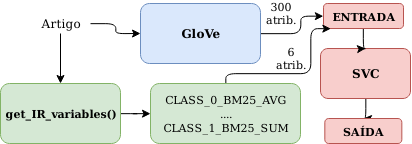
\includegraphics[width=0.68\textwidth]{img/4-tom-arquitetura-com-ri.png}
    \end{center}
    \vspace{-0.5cm}
    \legend{\ABNTEXfontereduzida \textbf{Fonte:} O autor.}
    \label{fig:4-tom-arquitetura-com-ri}
\end{figure}

				Para adicionar os 6 atributos de RI estes foram calculados para os respectivos documentos e embutidos no vetor GloVe do documento, resultando em documentos representados por 306 dimensões, ou 306 atributos.
				A arquitetura da solução adaptada está ilustrada na Figura \ref{fig:4-tom-arquitetura-com-ri}.
				% \ref{fig:4-tom-arquitetura-com-ri}

		\subsection{Corpus DB\underscore{}AUTHORPROF}
			O corpus DB\underscore{}AUTHORPROF consiste de \textit{tweets} de autores em três línguas diferentes, inglês, espanhol e árabe.
			Para avaliação dos atributos de RI o escopo de melhoria de desempenho foram considerados somente os classificadores das soluções para os autores de língua inglesa, e as imagens não foram consideradas.

			O conjunto de treinamento de autores da língua inglesa consiste de 300 mil \textit{tweets} de 3000 autores diferentes, e como o conjunto de validação final está disponível ao público, necessário somente solicitar o acesso, não foi necessário fazer o \textit{holdout} do conjunto de treinamento.
			O conjunto de validação da língua inglesa consiste de 190 mil tweets de 1900 autores.

			Os 300 mil \textit{tweets} foram indexados em todas as ferramentas de indexação permitindo a geração dos atributos de RI posteriormente para cada \textit{tweet} específico.

			\subsubsection{Solução 2\underscore{}daneshvar18}
			% baseou o seu pré-processamento em soluções das melhores equipes dos anos anteriores em tarefas da PAN CLEF
			%  O QUE É N-GRAM
				A solução de \citeonline{daneshvar:2018} utilizou um classificador SVM com diferentes tipos de $n$-grams de palavras e caracteres como atributos, e o melhor resultado obtido foi com a criação dos $n$-grams, posterior redução de dimensionalidade e então utilização do classificador LinearSVC da biblioteca sklearn para Python para criar o modelo de classificação.

				A adaptação da solução para adicionar os atributos de RI poderia ser feita adicionando os atributos antes ou depois da redução de dimensionalidade utilizada pela equipe.
				Os documentos inicialmente são representados por vetores de 1243271 dimensões, após a diminuição da dimensionalidade cada documento é representado por um vetor de 300 dimensões.
				No entanto, uma peculiaridade da solução está em como é feita a classificação, os 100 \textit{tweets} de cada autor são tratados como um único documento, pois o objetivo é classificar o gênero dos autores em homens ou mulheres.
				Como os \textit{tweets} foram indexados individualmente, então para adicionar os atributos de RI para cada autor foi feita a geração dos 6 atributos para todos os tweets e então estes foram agregados por autor.
				A arquitetura adaptada do sistema pode ser vista na Figura \ref{fig:2-daneshvar18-arquitetura-com-ri}.

				\begin{figure}[ht]
    \centering
    \caption{Arquitetura de sistema da solução 2\underscore{}daneshvar18 após adaptação.}
    \begin{center}
        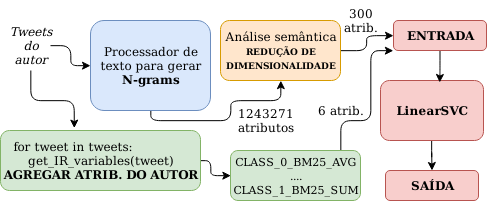
\includegraphics[width=0.75\textwidth]{img/2-daneshvar18-arquitetura-com-ri.png}
    \end{center}
    \vspace{-0.5cm}
    \legend{\ABNTEXfontereduzida \textbf{Fonte:} O autor.}
    \label{fig:2-daneshvar18-arquitetura-com-ri}
\end{figure}

				% Por fim, os 6 atributos de RI agregados por autor foram embutidos ao final da representação dos documentos, resultando em documentos representados por 1243277 dimensões, e posteriormente também foi configurado outro experimento para embutir os atributos de RI somente após a redução de dimensionalidade, resultando em documentos represetados por 306 atributos.
				Por fim, os 6 atributos de RI agregados por autor foram embutidos ao final da representação dos documentos após a redução de dimensionalidade, resultando em documentos represetados por 306 atributos.


		\subsection{Resumo das soluções} \label{sec:ResumoDasSoluções}
			Na Tabela \ref{tab:resumo-soluções} a seguir estão as principais características das soluções selecionadas.

			\begin{table}[!thb]
	%\huge
    \centering
    \caption{Resumo dos detalhes das soluções selecionadas.}
    \begin{adjustbox}{max width={\textwidth},keepaspectratio}%
    \begin{tabular}{|l|c|c|c|c|c|}
        % \toprule
        \hline
        \textbf{Solução}
        & \textbf{Pré-processamento} & \textbf{Núm. atrib.} & \textbf{Redução dim.} 
        & \textbf{Núm. atrib. após}  & \textbf{Classificador}
        \\ \hline
        1\underscore{}bertha        
        & ELMo          & 200 x 1024        & Não
        & 200 x 1024    & CNN (5 cam. esc.) 
        \\ \hline
        4\underscore{}tom
        & GloVe         & 300               & Não
        & 300           & SVC                
        \\ \hline
        2\underscore{}daneshvar18
        & N-gram palavras+caracteres & 1243271           & Sim
        & 300           & LinearSVC          
        \\ 
        \hline
        % \bottomrule
    \end{tabular}
    \end{adjustbox}
    \legend{\ABNTEXfontereduzida \textbf{Fonte:} O autor.}
    \label{tab:resumo-soluções} 
    % \legend{\textbf{Fonte:} O autor.}
\end{table}


	\section{Desempenho das ferramentas de armazenamento e indexação} \label{sec:DesempenhoFerramentas}
		Para cálculo das medidas TIME\underscore{}INDEX e TIME\underscore{}QUERY, conforme sugeridas no Capítulo \ref{ch:MateriaisMétodos}, foi empregada a linguagem de programação Python, utilizada para implementada uma classe chamada \textit{IndexToolManager} que abstrai a indexação e o cálculo das variáveis de RI com as ferramentas. 

		Essa classe foi central para todo o estudo, a utilização dela concentrou as funções para acesso e manipulação, quando disponíveis, aos dados das ferramentas de armazenamento e indexação, centralização das diferentes bibliotecas do Python já disponíveis para interagir com o ArangoDB e com o Elasticsearch, python-arango e elasticsearch-py respectivamente. 
		Trechos da implementação da classe \textit{IndexToolManager} estão no Apêndice \ref{apên:implementação-indextoolmanager}.
		% Adicionar funcṍes importantes e citar código aqui?
		\subsection{Tempo de indexação}
			Para cálculo da medida TIME\underscore{}INDEX foi criado um script Python nomeado \texttt{time\underscore{}index.py}, o qual utilizou da classe \textit{IndexToolManager} em duas funções feitas para executar a indexação dos bancos de dados, DB\underscore{}AUTHORPROF e DB\underscore{}HYPERPARTISAN, nas 3 ferramentas, ArangoDB, Elasticsearch e Zettair.
			A função principal do script \texttt{time\underscore{}index.py} possui nome \textit{measure\underscore{}TIME\underscore{}INDEX}, e um trecho do código que implementa essa função pode ser visto a seguir no Código \ref{cmd:function-measure-time-index}.

			\sourcecodenolinenos{Função \textit{measure\underscore{}TIME\underscore{}INDEX} do script \texttt{time\underscore{}index.py}.}{function-measure-time-index}{python}{function-measure-TIME-INDEX.py}
			% \sourcecodeinline{python}{codes/function-measure-TIME-INDEX.py}

			Essa função é responsável por efetuar uma chamada à função \textit{index} com os parâmetros de tipo de indexação, corpus a ser indexado, e qual a ferramenta utilizada nessa indexação, além de uma identificação do experimento.
			A função \textit{index}, que pode ser vista no Apêndice \ref{apên:função-index}, faz os devidos tratamentos para chamar os métodos da classe \textit{IndexToolManager} responsáveis por fazer a indexação dos documentos do corpus especificado utilizando a ferramenta especificada, isso enquanto mensura o tempo que cada indexação levou e registra todas as operações num arquivo de texto.

			% Colocar o código fonte da função index aqui?
			
			Como as ferramentas ArangoDB e Elasticsearch se assemelham bastante a sistemas gerenciadores de bancos de dados completos, preparados, inclusive, para distribuição geográfica dos dados, há de ser citada essa grande diferença deles para o Zettair, este último que é somente um sistema para indexação em lotes e consulta local dos dados, não permitindo, por exemplo, adição de novos documentos em um índice. 
			A ação de inserção unitária é um procedimento comum em SGBDs. 			

			A operação de indexação foi executada de dois modos, em lote e unitária, sendo que o Zettair só permite a inserção em lote. 
			Na Figura \ref{fig:time-index-bulk} pode ser visto o tempo mensurado, em milissegundos gastos por documento, para inserção em lote dos documentos dos corpus em cada ferramenta.

			\begin{figure}[h]
    \centering
    \caption{Medidas de desempenho TIME\_INDEX mensuradas para as ferramentas de armazenamento e indexação, com inserções feitas em lote.}
    \begin{center}
        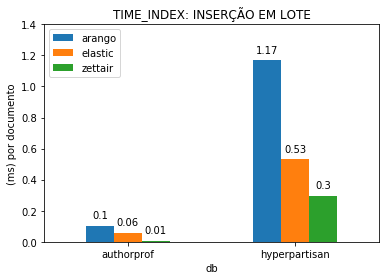
\includegraphics[width=0.75\textwidth]{img/time-index-bulk.png}
    \end{center}
    \vspace{-0.5cm}
    \legend{\ABNTEXfontereduzida \textbf{Fonte:} O autor.}
    \label{fig:time-index-bulk}
\end{figure}

			O Zettair é a ferramenta mais rápida para completar a indexação de ambos os corpus selecionados, levando somente 2,29 segundos para indexar os 300 mil documentos do corpus DB\underscore{}AUTHORPROF, menos de 0,01 milissegundos por documento.
			Dentre os SGBDs avaliados, o Elasticsearch supera o ArangoDB para inserções em lote, gastando 17,61 segundos para indexar os 300 mil \textit{tweets}, cerca de 0,06 milissegundos por documento.
			Nota-se ainda que a indexação do corpus DB\underscore{}HYPERPARTISAN é mais lenta quando se considera o tempo por documento inserido, porque, apesar do corpus DB\underscore{}AUTHORPROF ter um número bem maior de documentos, 300 mil em comparação com 645, cada artigo do DB\underscore{}HYPERPARTISAN é bem mais extenso que qualquer dos \textit{tweets} do DB\underscore{}AUTHORPROF.
			A mesma relação de velocidade entre as ferramentas observada para as inserções feitas com os documentos do DB\underscore{}AUTHORPROF se mantem para as inserções feitas com os documentos do DB\underscore{}HYPERPARTISAN, o Zettair é o mais rápido, e, dentre os SGBDs, o Elasticsearch é mais rápido que o ArangoDB.
			
			Para operação de inserção unitária, avaliada somente com o ArangoDB e Elasticsearch, foi levado em conta o tempo total para indexação de todos os documentos de cada corpus, inseridos em sequência, e posteriormente esses valores mensurados foram divididos pelo número de documentos.
			Na Figura \ref{fig:time-index-individual} estão dispostos os tempos totais para indexação de todos os documentos dos corpus com ambas as ferramentas. 

			\begin{figure}[h]
    \centering
    \caption{Medidas de desempenho TIME\_INDEX mensuradas para as ferramentas de armazenamento e indexação, com inserções unitárias.}
    \begin{center}
        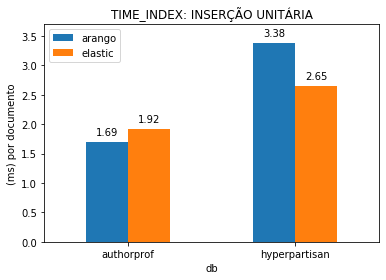
\includegraphics[width=0.75\textwidth]{img/time-index-individual.png}
    \end{center}
    \vspace{-0.5cm}
    \legend{\ABNTEXfontereduzida \textbf{Fonte:} O autor.}
    \label{fig:time-index-individual}
\end{figure}

			O ArangoDB teve um melhor desempenho para as inserções dos documentos do DB\underscore{}AUTHORPROF, com 1,69 milissegundos por documento, em contraste aos 1,92 milissegundos por documento do Elasticsearch.
			Porém, o Elasticsearch foi mais rápido para inserção dos documentos do DB\underscore{}HYPERPARTISAN, com 2,65 milissegundos por documento contra 3,38 milissegundos por documento do ArangoDB.		

			Percebe-se então que o ArangoDB se saiu um pouco melhor que o Elasticsearch na inserção de grande quantidade de documentos pequenos em sequência, evidenciado pelos tempos de inserção unitária da Figura \ref{fig:time-index-individual}.
			E pode-se supor que isto é derivado de alguma sobrecarga na operação de inserção unitária do Elasticsearch, ou talvez no custo de recálculo do índice que varia com o tamanho dos documentos inseridos, porém com um custo inicial maior, já que para inserção unitária dos documentos do DB\underscore{}HYPERPARTISAN, que são artigos extensos, o Elasticsearch teve melhor desempenho.
				
			No geral, o desempenho da indexação por inserção unitária fica abaixo da por inserção em lotes, como era esperado.

		\subsection{Tempo de consulta}
			Para medir o TIME\underscore{}QUERY utilizando cada ferramenta durante a execução das soluções foi necessário adaptar os códigos das soluções para fazer o registro do tempo que cada consulta, e posterior geração dos atributos de RI, levou.

			A fim de facilitar a geração dos atributos, foram implementados métodos na classe \textit{IndexToolManager} para que: dado um texto, seja cálculo direto das variáveis de RI já com as ferramentas específicas, como por exemplo o método \textit{arango\underscore{}get\underscore{}IR\underscore{}variables}.
			A utilização desses métodos pode ser visto no trecho disposto a seguir do script Python \texttt{feat\underscore{}GloVe.ipynb} da solução 4\underscore{}tom adaptada.

			% \sourcecodenolinenos{Trecho da adaptação feita ao script \texttt{feat\underscore{}GloVe.ipynb} da solução 4\underscore{}tom.}{time-query-calculation-4-tom}{python}{time-query-calculation-4-tom.py}
			\begin{listing}[H]
				\refstepcounter{sourcecode}
				\captionof{listing}{Trecho da adaptação feita ao script \texttt{feat\underscore{}GloVe.ipynb} da solução 4\underscore{}tom.\label{cmd:time-query-calculation-4-tom}}
			\end{listing}
			\vspace{-1.0cm}
			\inputminted[bgcolor=bg, 
			tabsize=4, baselinestretch=1, breaklines]{python}{codes/time-query-calculation-4-tom.py}
			\vspace{-1.0cm}
			\Ididthis

			Neste trecho, Código \ref{cmd:time-query-calculation-4-tom}, \textit{toolTest} é uma instância da classe \textit{IndexToolManager} com \textit{top-$k$} igual a 100. 
			Esta classe que é responsável pelo cálculo das variáveis de RI, e o tempo de consulta leva em conta esse cálculo, como fica exposto pela posição das variáveis \textit{initial} e \textit{final}.

			O mesmo tipo de adaptação feito para a solução 4\underscore{}tom foi feito para as demais, e as medidas coletadas estão dispostas na Figura \ref{fig:time-query}.

			\begin{figure}[h]
    \centering
    \caption{Medidas de desempenho TIME\_QUERY mensuradas para consulta e criação dos 6 atributos de RI sugeridos, utilizando as ferramentas de armazenamento e indexação.}
    \vspace{-0.5cm}
    \begin{center}
        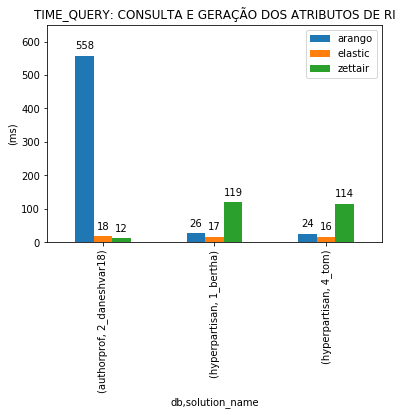
\includegraphics[scale=0.75]{img/time-query.png}
    \end{center}
    \vspace{-0.5cm}
    \legend{\ABNTEXfontereduzida \textbf{Fonte:} O autor.}
    \label{fig:time-query}
\end{figure}

			% Zettair, colocar detalhe dos modos de operação para consulta, iterativa e consulta única

			Ao ver os resultados percebe-se uma discrepância entre os resultados do Zettair nos dois corpus, levando somente 12 milissegundos para o cálculo dos atributos de RI no corpus  corpus DB\underscore{}AUTHORPROF e mais de 110 milissegundos para as soluções do corpus DB\underscore{}HYPERPARTISAN.
			Isso acontece pois o Zettair possui dois modos de operação para consultas, o 
			\begin{enumerate*}[label=(\alph*)]
				\item modo iterativo e o 
				\item modo de consulta única
			\end{enumerate*}.
			Em ambos os modos o Zettair efetua uma etapa de inicialização, copiando o índice gerado para a memória, e para efetuar consultas em série o modo iterativo é o ideal, no entanto ele possui uma limitação não documentada de cerca de 2048 caracteres nas consultas, como no corpus DB\underscore{}AUTHORPROF todos os documentos são pequenos, portanto menores que esse limite, as consultas para gerar os atributos de RI com o Zettair puderam ser executadas no modo iterativo.
			No entanto, para o corpus DB\underscore{}HYPERPARTISAN isso não foi possível pois diversos  documentos ultrapassam essa limitação de 2048 caracteres, portanto, para este corpus, as consultas realizadas com o Zettair utilizaram o modo de consulta única.

			A outra surpresa foi o ArangoDB, que levou 558 milissegundos para efetuar cada consulta no corpus DB\underscore{}AUTHORPROF, o que indica que seu algoritmo para cálculo do BM25 tem um custo de desempenho proporcional ao número de documentos indexados no banco de dados, pois o corpus DB\underscore{}AUTHORPROF possui 300 mil documentos indexados, e o DB\underscore{}HYPERPARTISAN somente 430.
			Enquanto isso, o Elasticsearch teve desempenho similar para cálculo dos atributos de RI nos dois corpus, chegando no máximo a 18 milissegundos por consulta no corpus DB\underscore{}AUTHORPROF.

			O Zettair é a ferramenta mais rápida para a consulta e geração dos atributos de RI no corpus DB\underscore{}AUTHORPROF, porém o Elasticsearch é a melhor ferramenta, em quesito geral de tempo de consulta, devido à limitação do tamanho de documento do modo iterativo do Zettair.

	\section{Desempenho dos classificadores com atributos de RI} \label{sec:DesempenhoClassificadores}
		O desempenho dos classificadores foi mensurado conforme as medidas CLF\underscore{}ACC e CLF\underscore{}F1 estabelecidas na Subseção \ref{subsec:Desempenho-de-classificador} do Capítulo \ref{ch:MateriaisMétodos}, esses valores foram coletados reproduzindo as soluções originais e então reproduzindo as soluções com as adaptações para incluir os atributos de RI gerados por cada uma das ferramentas.

		A seguir são apresentados as medidas coletadas para as soluções dos corpus.

		\subsection{DB\underscore{}HYPERPARTISAN}
			Antes da adaptação das soluções selecionadas foi necessário reproduzi-las, no entanto, como o conjunto de validação da competição de 628 não foi disponibilizado ao público e foi necessário fazer o \textit{holdout} no conjunto de treinamento, não é possível comparar diretamente os resultados finais divulgados na página da competição com os obtidos.
			Pois, para submissão dos classificadores finais para a da competição, ambas as soluções 1\underscore{}bertha e 4\underscore{}tom treinaram seus classificadores com os 645 artigos e os resultados de acurácia e $F_1$-score disponíveis no ranking da competição foram calculados para as predições feitas nos 628 exemplos do conjunto de validação.
			Além disso, outro problema é que o script Python da solução 1\underscore{}bertha disponibilizado online não possuia números aleatórios fixos, o que torna praticamente impossível reproduzir a mesma solução que foi submetida pela equipe para a competição.

			Encontram-se na Tabela \ref{tab:reprodução-db-hyperpartisan} as medidas divulgadas na página da competição \textit{SemEval 2019} \cite{PAN_HNDLEADERBOARD_2019} e as reproduções feitas com treinamento em 430 artigos e validação nos 215 restantes.

			\begin{table}[!thb]
	%\huge
    \centering
    \caption{Comparação das medidas das soluções do corpus DB\underscore{}HYPERPARTISAN divulgadas pelas competição e das reproduções.}
    \begin{adjustbox}{max width={\textwidth},keepaspectratio}%
    \begin{tabular}{|l|c|c|c|c|c|}
        % \toprule
        \hline
        \multirow{2}{*}{\textbf{Solução}}
        & \multicolumn{2}{|c|}{\textbf{Acurácia}}
        & \multicolumn{2}{|c|}{\textbf{$F_1$-score}}
        \\ \cline{2-5}    
        & Competição    & Reprodução
        & Competição    & Reprodução 
        \\ \hline
        1\underscore{}bertha        
        & 0,822         & 0,814
        & 0,809         & 0,762
        \\ \hline
        4\underscore{}tom
        & 0,806         & 0,809
        & 0,790         & 0,707              
        \\ 
        \hline
        % \bottomrule
    \end{tabular}
    \end{adjustbox}
    \legend{\ABNTEXfontereduzida \textbf{Fonte:} O autor.}
    \label{tab:reprodução-db-hyperpartisan} 
    % \legend{\textbf{Fonte:} O autor.}
\end{table}


			Após essa validação que não há nada de muito errado com as soluções reproduzidas em comparação com os resultados divulgados pela competição, pois os resultados reproduzidos ficam dentro do esperado para um conjunto de treinamento reduzido, as soluções foram adaptadas para incluir os atributos de RI conforme o descrito nas seções anteriores.
			Na Figura \ref{fig:clf-acc-bars-hyperpartisan} estão dispostas as medidas CLF\underscore{}ACC para ambas as soluções.
			
			\begin{figure}[h]
    \centering
    \caption{Desempenho CLF\_ACC das soluções do corpus DB\_HYPERPARTISAN.}
    \vspace{-0.5cm}
    \begin{center}
        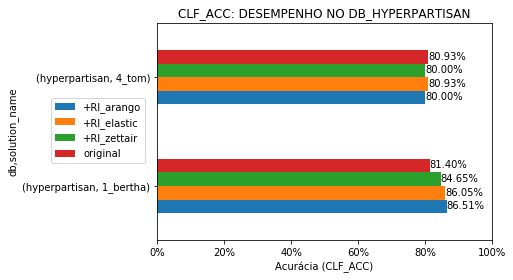
\includegraphics[scale=0.75]{img/clf-acc-bars-hyperpartisan.png}
    \end{center}
    \vspace{-0.5cm}
    \legend{\ABNTEXfontereduzida \textbf{Fonte:} O autor.}
    \label{fig:clf-acc-bars-hyperpartisan}
\end{figure}

			E na Figura \ref{fig:clf-f1-bars-hyperpartisan} estão dispostas as medidas CLF\underscore{}F1.
			
			\begin{figure}[h]
    \centering
    \caption{Desempenho CLF\_F1 das soluções do corpus DB\_HYPERPARTISAN.}
    \vspace{-0.5cm}
    \begin{center}
        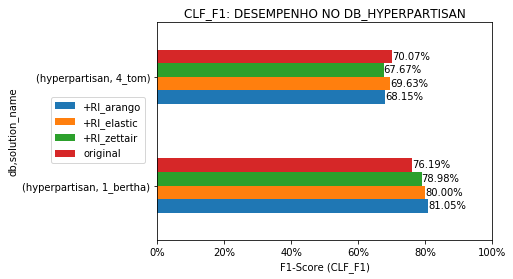
\includegraphics[scale=0.75]{img/clf-f1-bars-hyperpartisan.png}
    \end{center}
    \vspace{-0.5cm}
    \legend{\ABNTEXfontereduzida \textbf{Fonte:} O autor.}
    \label{fig:clf-f1-bars-hyperpartisan}
\end{figure}

			A adição dos atributos de RI proporciona ganho de acurácia e também de $F_1$-Score para a solução 1\underscore{}bertha, alcançando valores maiores até mesmo que os finais da competição com acurácia de $0,8651$ ($86,51\%$) e $F_1$-Score de $0,8105$ ($81,05\%$) quando adicionados os atributos de RI gerados pelo ArangoDB.
			Já para a solução 4\underscore{}tom inicialmente a adição dos atributos de RI não proporciona nenhum ganho de acurácia ou $F_1$-Score, pelo contrário, com todas as ferramentas o $F_1$-Score foi menor ao adicionar os atributos de RI, e somente com os atributos de RI do Elasticsearch que a acurácia se manteve a mesma, com o ArangoDB e com o Zettair houve também diminuição da acurácia do classificador da solução 4\underscore{}tom.

			Deve ser observado um detalhe importante da solução 4\underscore{}tom, que é o classificador utilizado e o modo escolhido para definição dos parâmetros desse classificador pela equipe, que no caso foi o classificador SVC e na elaboração de sua solução a equipe avaliou diferentes valores do parâmetro C do classificador e escolheu o valor de C com melhor resultado nesse teste, que foi $C = 0,9$.
			Como o conjunto de treinamento para submissão da equipe consistiu de todos os 645 artigos, e na reprodução feita para este estudo isso não pode ser feito devido à necessidade de um conjunto isolado de validação, foi feita a suposição que o melhor valor de C para a reprodução da solução seria diferente, pois o conjunto de treinamento da reprodução possui somente 430 artigos.
			
			Nas Figuras \ref{fig:clf-acc-4-tom} e \ref{fig:clf-f1-4-tom} estão plotadas as medidas CLF\underscore{}ACC e CLF\underscore{}F1 obtidas com a reprodução da solução 4\underscore{}tom com valores de C na faixa de 0,00001 a 10,0.
			
			\begin{figure}[h]
    \centering
    \caption{Desempenho CLF\_ACC da solução 4\_tom para diferentes valores de refinamento da função custo, parâmetro C do classificador SVC.}
    \vspace{-0.5cm}
    \begin{center}
        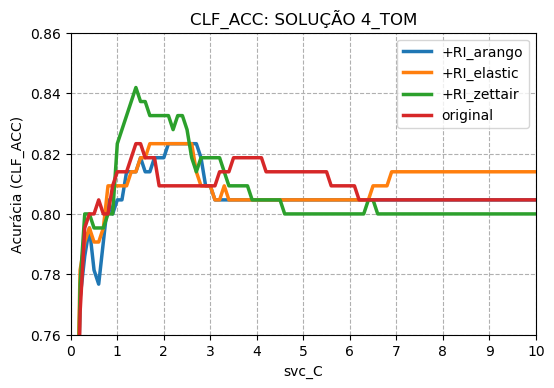
\includegraphics[scale=0.75]{img/clf-acc-4-tom.png}
    \end{center}
    \vspace{-0.5cm}
    \legend{\ABNTEXfontereduzida \textbf{Fonte:} O autor.}
    \label{fig:clf-acc-4-tom}
\end{figure}

			\begin{figure}[h]
    \centering
    \caption{Desempenho CLF\_F1 da solução 4\_tom para diferentes valores de refinamento da função custo, parâmetro C do classificador SVC.}
    \vspace{-0.5cm}
    \begin{center}
        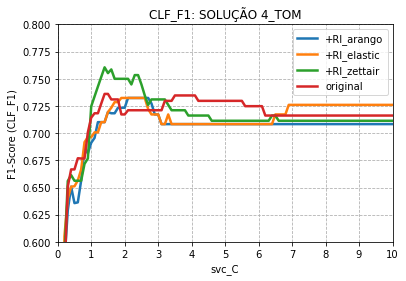
\includegraphics[scale=0.75]{img/clf-f1-4-tom.png}
    \end{center}
    \vspace{-0.5cm}
    \legend{\ABNTEXfontereduzida \textbf{Fonte:} O autor.}
    \label{fig:clf-f1-4-tom}
\end{figure}
			
			Uma rápida análise dos gráficos permite perceber que os melhores valores do parâmetro C agora se encontram na faixa de 1,0 a 3,0 para as reproduções, tanto em termos de CLF\underscore{}ACC quanto de CLF\underscore{}F1.
			O valor de $C = 0,9$ de fato não está entre os melhores possíveis para o classificador.
			
			Nota-se que, mesmo com a adição dos atributos de RI, utilizando tanto o ArangoDB quanto o Elasticsearch, o classificador em nenhum momento consegue superar o melhor valor de C do classificador original, porém, com adição dos atributos de RI gerados pelo Zettair, ele atinge os valores de $\text{CLF\underscore{}ACC} = 0,8419$ e $\text{CLF\underscore{}F1} = 0,7606$ quando $C = 1,4$.
			Os valores máximos atingidos com os respectivos valores de C estão dispostos na Tabela \ref{tab:reprodução-4-tom-c}.

			\begin{table}[!thb]
	%\huge
    \centering
    \caption{Melhores valores de CLF\underscore{}ACC e CLF\underscore{}F1 do classificador SVC da solução 4\underscore{}tom após reproduzida com diferentes valores de C.}
    \begin{adjustbox}{max width={\textwidth},keepaspectratio}%
    \begin{tabular}{|l|c|c|c|}
        % \toprule
        \hline
        \textbf{Solução}
        & \textbf{C}
        & \textbf{Acurácia}
        & \textbf{$F_1$-score}
        \\ \hline
        original        
        & 1,4   & 0,8233   & 0,7361 
        \\ \hline
        +RI\underscore{}arango
        & 2,1   & 0,8233    & 0,7324          
        \\ \hline
        +RI\underscore{}elastic
        & 1,9   & 0,8233    & 0,7324        
        \\ \hline
        +RI\underscore{}zettair
        & 1,4   & \textbf{0,8419}    & \textbf{0,7606}          
        \\ 
        \hline
        % \bottomrule
    \end{tabular}
    \end{adjustbox}
    \legend{\ABNTEXfontereduzida \textbf{Fonte:} O autor.}
    \label{tab:reprodução-4-tom-c} 
    % \legend{\textbf{Fonte:} O autor.}
\end{table}


			Observa-se então que a adição dos atributos de RI, utilizando o Zettair para gerá-los, oferece um ganho de desempenho para o classificador SVC da solução 4\underscore{}tom quando efetuada a otimização de hiperparâmetros.
			Porém, ainda assim o classificador SVC não consegue superar os resultados obtidos com o classificar CNN da solução 1\underscore{}bertha ao adicionar os parâmetros de RI com quaisquer das ferramentas.
			O que pode parecer um tanto estranho, já que na solução 4\underscore{}tom somente o Zettair produziu ganho de desempenho do classificador.
			Talvez isso esteja relacionado ao modo de classificação final utilizado pela solução 1\underscore{}bertha, no qual é feito o \textit{ensemble} (junção) dos três melhores modelos de qualquer época durante o treinamento da CNN, é possível que os atributos de RI não sejam os responsáveis pelo ganho de desempenho observado na solução 1\underscore{}bertha, mas somente a iteração diferente, devido a alteração no conjunto de atributos feita por cada ferramenta, tenha gerado modelos que tenham melhor desempenho no \textit{ensemble}.
			% Nota de rodapé sobre ensemble?
			Pois, mesmo com a fixação da semente do gerador de número aleatório, como os valores dos atributos de RI são alterados (já que cada ferramenta sua própria implementação do BM25 com pequenas diferenças entre si), os modelos gerados pela reprodução com adição dos atributos de RI gerados pelo Zettair é diferente dos gerados pelo Elasticsearch, que também é diferente dos gerados pelo ArangoDB, e todos estes também são diferentes dos modelos gerados sem adição dos atributos de RI.


		\subsection{DB\underscore{}AUTHORPROF}
			A solução 2\underscore{}daneshvar18 foi reproduzida sem nenhuma adaptação para comparação com os valores que se encontram na página da competição.
			Na Tabela \ref{tab:reprodução-db-authorprof} está a medida de acurácia divulgada na página da competição \cite{PAN_APCLEF_2018} junto com as medidas da reprodução feitas do mesmo modo que a submissão original, treinamento com os tweets de 3000 autores de língua inglesa e validação com os tweets de 1900 autores de língua inglesa.
			% e a medida $F_1$-score apresentada na descrição da solução pela equipe
			% PAN_APCLEF_2018.

			\begin{table}[!thb]
	%\huge
    \centering
    \caption{Comparação das medidas da solução 2\underscore{}daneshvar18 do corpus DB\underscore{}AUTHORPROF divulgadas pela competição e da reprodução da solução.}
    \begin{adjustbox}{max width={\textwidth},keepaspectratio}%
    \begin{tabular}{|l|c|c|c|c|c|}
        % \toprule
        \hline
        \multirow{2}{*}{\textbf{Solução}}
        & \multicolumn{2}{|c|}{\textbf{Acurácia}}
        & \multicolumn{2}{|c|}{\textbf{$F_1$-score}}
        \\ \cline{2-5}    
        & Competição    & Reprodução
        & Competição    & Reprodução 
        \\ \hline
        2\underscore{}daneshvar18        
        & 0,8221        & 0,822105	
        & --            & 0,820785
        \\ 
        \hline
        % \bottomrule
    \end{tabular}
    \end{adjustbox}
    \legend{\ABNTEXfontereduzida \textbf{Fonte:} O autor.}
    \label{tab:reprodução-db-authorprof} 
    % \legend{\textbf{Fonte:} O autor.}
\end{table}


			Ao truncar o resultado de acurácia da solução reproduzida em 4 dígitos, confirmamos que o mesmo valor divulgado na página da competição é o obtido ao reproduzir a solução.
			Tanto a página da competição quanto o artigo de descrição da solução \cite{daneshvar:2018} só mencionam a acurácia da solução, portanto não há como comparar o $F_1$-score obtido ao reproduzir a solução.

			Depois da validação inicial da solução 2\underscore{}daneshvar por meio da reprodução dos resultados da competição, ela foi adaptada para incluir os atributos de RI junto aos atributos de entrada do classificador antes da redução de dimensionalidade.
			As medições de CLF\underscore{}ACC e CLF\underscore{}F1 obtidas ao reproduzir a solução incluindo os atributos com as diferentes ferramentas estão dispostas nas Figura \ref{fig:clf-bars-authorprof}.
			%  e \ref{fig:clf-f1-bars-authorprof}.

			\begin{figure}[ht]
    \centering
    \caption{Desempenho CLF\underscore{}F1 e CLF\underscore{}ACC da solução reproduzida para o corpus DB\underscore{}AUTHORPROF.}
    \vspace{-0.5cm}
    \begin{center}
        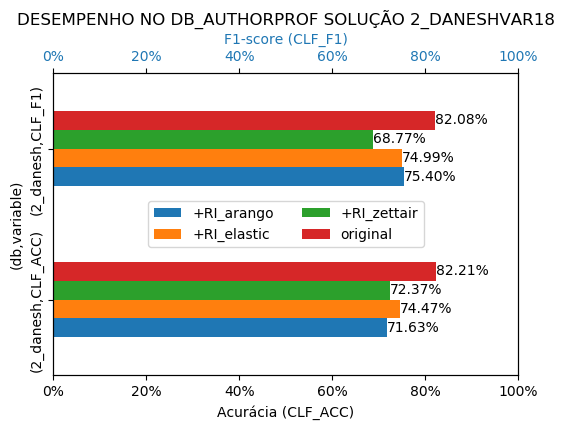
\includegraphics[scale=0.75]{img/clf-bars-authorprof.png}
    \end{center}
    \vspace{-0.5cm}
    \legend{\ABNTEXfontereduzida \textbf{Fonte:} O autor.}
    \label{fig:clf-bars-authorprof}
\end{figure}

			% \begin{figure}[ht]
    \centering
    \caption{Desempenho CLF\underscore{}ACC da solução reproduzida para o corpus DB\underscore{}AUTHORPROF.}
    \vspace{-0.5cm}
    \begin{center}
        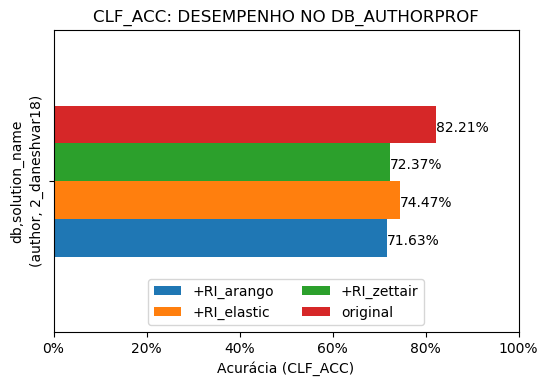
\includegraphics[scale=0.75]{img/clf-acc-bars-authorprof.png}
    \end{center}
    \vspace{-0.5cm}
    \legend{\ABNTEXfontereduzida \textbf{Fonte:} O autor.}
    \label{fig:clf-acc-bars-authorprof}
\end{figure}


			% \begin{figure}[h]
    \centering
    \caption{Desempenho CLF\_F1 da solução reproduzida para o corpus DB\_AUTHORPROF.}
    \vspace{-0.5cm}
    \begin{center}
        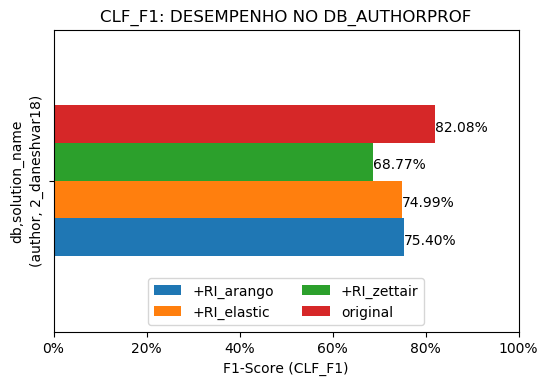
\includegraphics[scale=0.75]{img/clf-f1-bars-authorprof.png}
    \end{center}
    \vspace{-0.5cm}
    \legend{\ABNTEXfontereduzida \textbf{Fonte:} O autor.}
    \label{fig:clf-f1-bars-authorprof}
\end{figure}

			Como pode ser observado nos gráficos, os atributos de RI na verdade provocaram uma perda considerável de desempenho do classificador da solução 2\underscore{}daneshvar18, ambas as medidas CLF\underscore{}ACC e CLF\underscore{}F1 foram menores com a adição dos atributos de RI com quaisquer das ferramentas utilizadas.
			O classificador da solução se trata de um classificador do tipo de Máquinas de Vetor de Suporte, o LinearSVC, e assim como foi feito com a solução 4\underscore{}tom anteriormente, pode-se supor que o parâmetro C do classificador, escolhido como o padrão $C = 1,0$ pela equipe da solução 2\underscore{}daneshvar18, não se trata do melhor valor possível para os modelos de classificação gerados ao adicionar os atributos de RI.
			Então, trabalhando com essa hipótese, a solução foi reproduzida alterando o valor de C do LinearSVC na faixa de valores de $0,00001$ a $10,0$.
			As medidas coletadas estão plotadas nas Figuras \ref{fig:clf-acc-2-daneshvar18} e \ref{fig:clf-f1-2-daneshvar18}.


			\begin{figure}[ht]
    \centering
    \caption{Desempenho CLF\underscore{}ACC da solução 2\underscore{}daneshvar18 para diferentes valores de refinamento da função custo, parâmetro C do classificador LinearSVC.}
    \vspace{-0.5cm}
    \begin{center}
        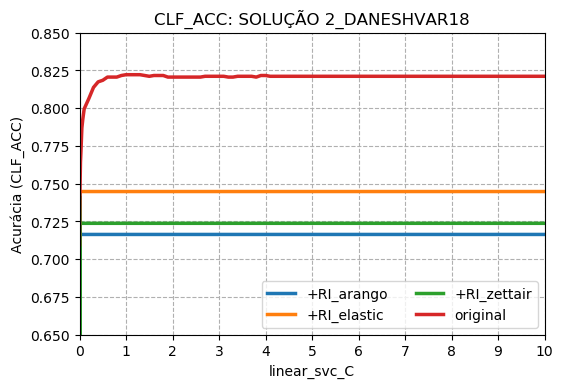
\includegraphics[scale=0.75]{img/clf-acc-2-daneshvar18.png}
    \end{center}
    \vspace{-0.5cm}
    \legend{\ABNTEXfontereduzida \textbf{Fonte:} O autor.}
    \label{fig:clf-acc-2-daneshvar18}
\end{figure}

			\begin{figure}[ht]
    \centering
    \caption{Desempenho CLF\underscore{}F1 da solução 2\underscore{}daneshvar18 para diferentes valores de refinamento da função custo, parâmetro C do classificador LinearSVC.}
    \vspace{-0.5cm}
    \begin{center}
        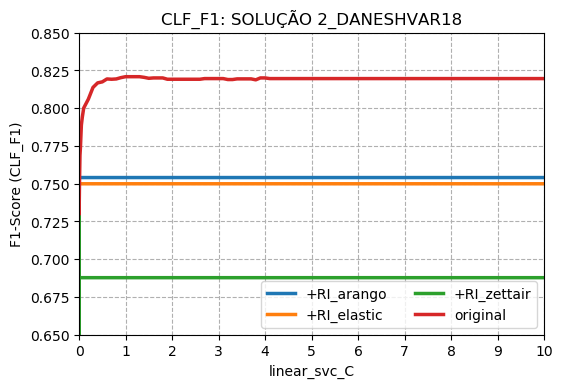
\includegraphics[scale=0.75]{img/clf-f1-2-daneshvar18.png}
    \end{center}
    \vspace{-0.5cm}
    \legend{\ABNTEXfontereduzida \textbf{Fonte:} O autor.}
    \label{fig:clf-f1-2-daneshvar18}
\end{figure}

			Os gráficos de desempenho com diferentes valores de C comprovam que os atributos de RI pioraram os modelos gerados pelo classificador LinearSVC da solução 2\underscore{}daneshvar18.
			Pode-se dizer que a introdução dos atributos de RI se trata de uma introdução de ruído que atrapalha o classificador e o impede alcançar os níveis de desempenho atingidos utilizando somente os atributos originais.

			Por que isso ocorreu?
			Ao analisar os atributos originais após a redução de dimensionalidade foi constatado que os valores máximos e mínimos de cada uma das colunas dos 300 atributos estavam na faixa de $-1,0$ a $1,0$ enquanto que os 6 atributos de RI gerados pelas ferramentas estavam na faixa de $8,0$ até a casa dos milhares.
			Os classificadores do tipo SVM atribuem maior importância a atributos com maiores magnitudes conforme o núcleo selecionado \cite{Kumar2014}, e isso estava acontecendo com o núcleo padrão do classificador LinearSVC do sklearn.

			Para tentar resolver o problema foi utilizado o escalonador MinMaxScaler nos 6 atributos de RI para dimensioná-los para a faixa de $-1,0$ a $1,0$. 
			Os medidas coletadas podem ser observadas nas Figuras \ref{fig:clf-acc-2-daneshvar18-ir-scaled} e \ref{fig:clf-f1-2-daneshvar18-ir-scaled}. 

			\begin{figure}[h]
    \centering
    \caption{Desempenho CLF\_ACC da solução 2\_daneshvar18 para diferentes valores de refinamento da função custo, parâmetro C do classificador LinearSVC com atributos de RI escalonados pelo MinMaxScaler.}
    \vspace{-0.5cm}
    \begin{center}
        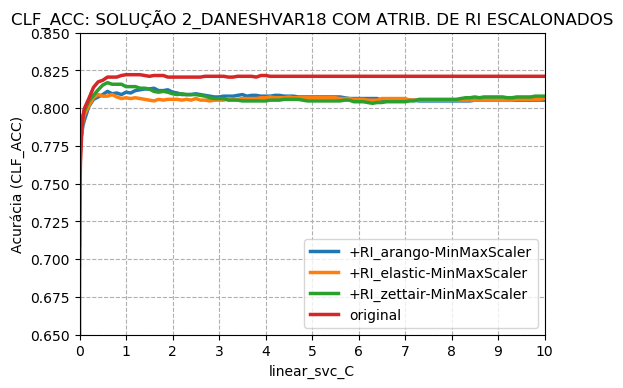
\includegraphics[scale=0.75]{img/clf-acc-2-daneshvar18-ir-scaled.png}
    \end{center}
    \vspace{-0.5cm}
    \legend{\ABNTEXfontereduzida \textbf{Fonte:} O autor.}
    \label{fig:clf-acc-2-daneshvar18-ir-scaled}
\end{figure}

			\begin{figure}[h]
    \centering
    \caption{Desempenho CLF\_F1 da solução 2\_daneshvar18 para diferentes valores de refinamento da função custo, parâmetro C do classificador LinearSVC com atributos de RI escalonados pelo MinMaxScaler.}
    \vspace{-0.5cm}
    \begin{center}
        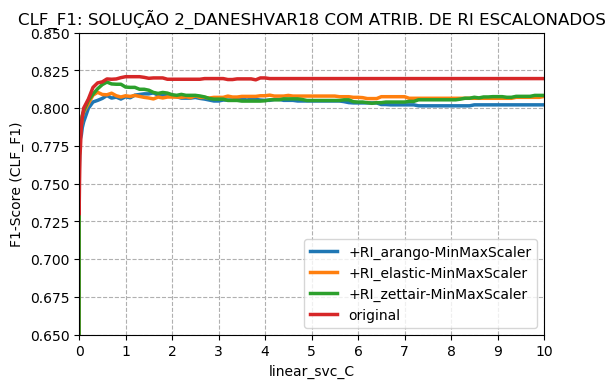
\includegraphics[scale=0.75]{img/clf-f1-2-daneshvar18-ir-scaled.png}
    \end{center}
    \vspace{-0.5cm}
    \legend{\ABNTEXfontereduzida \textbf{Fonte:} O autor.}
    \label{fig:clf-f1-2-daneshvar18-ir-scaled}
\end{figure}

			Apesar do desempenho do classificador da solução 2\underscore{}daneshvar18 ter sido maior com os atributos de RI escalonados, como mostra o gráfico da Figura \ref{fig:clf-acc-2-daneshvar18-ir-scaled} em comparação com o da Figura \ref{fig:clf-acc-2-daneshvar18}, ainda assim o desempenho continuou abaixo da reprodução da solução original.
			Na Tabela \ref{tab:reprodução-2-daneshvar18-c} podem ser vistos os valores máximos atingidos com os respectivos valores de C.

			\begin{table}[!thb]
	%\huge
    \centering
    \caption{Melhores valores de CLF\_ACC e CLF\_F1 do classificador LinearSVC da solução 2\_daneshvar18 após reproduzida com diferentes valores de C, com atributos de RI escalonados pelo MinMaxScaler.}
    \begin{adjustbox}{max width={\textwidth},keepaspectratio}%
    \begin{tabular}{|l|c|c|c|}
        % \toprule
        \hline
        \textbf{Solução}
        & \textbf{C}
        & \textbf{Acurácia}
        & \textbf{$F_1$-Score}
        \\ \hline
        original        
        & 1,0   & \textbf{0,822105}   & \textbf{0,820785}
        \\ \hline
        +RI\_arango
        & 1,6   & 0,813158   & 0,810059          
        \\ \hline
        +RI\_elastic
        & 0,4   & 0,808947    & 0,810444
        \\ \hline
        +RI\_zettair
        & 0,6   & 0,816842	    & 0,817227
        \\ 
        \hline
        % \bottomrule
    \end{tabular}
    \end{adjustbox}
    \legend{\ABNTEXfontereduzida \textbf{Fonte:} O autor.}
    \label{tab:reprodução-2-daneshvar18-c} 
    % \legend{\textbf{Fonte:} O autor.}
\end{table}


			Pode-se perceber que o melhor desempenho com os atributos de RI é quando gerado pelo Zettair, no entanto ainda assim fica abaixo da solução original.
			Obtendo acurácia de $81,68\%$ contra $82,22\%$ da original, e $F_1$-score de $81,72\%$ contra $82,08\%$ da original.
	% Fluxograma das alterações feitas nos códigos com exemplos de trechos alterados
	% Rosalvo disse que é para colocar no Apêndice

	% ganho de informação das 6 variáveis nas soluções

	% Citar as técnicas só de um, descrições, citar algum livro ou página

	% Criar rede neural para comparar à solução do DB_AUTHORPROF à parte 

